\exercise{Optimal Control}
In this exercise, we consider a finite-horizon discrete time-varying Stochastic Linear Quadratic Regulator with Gaussian noise and time-varying quadratic reward function. Such system is defined as
%
\begin{align}
	\vec s_{t+1} = \mat A_t \vec s_t + \mat B_t \vec a_t + \vec w_t\,, 
\end{align}
where $\vec s_t$ is the state, $\vec a_t$ is the control signal, $\vec w_t \sim \gauss{\vec b_t}{\Sigma_t}$ is Gaussian additive noise with mean $\vec b_t$ and covariance $\Sigma_t$ and $t=0,1,\dots,T$ is the time horizon. 
The control signal $\vec a_t$ is computed as
%
\begin{align}
	\vec a_t = - \mat K_t \vec s_t + \vec k_t
\end{align}
%
and the reward function $r_t$ is
%
\begin{align}
	r_t = \begin{cases}
	- (\vec s_t - \vec r_t)\T \mat R_t (\vec s_t - \vec r_t) - \vec a\T_t \mat H_t \vec a_t  & \text{when \quad} t=0,1,\dots,T-1
	\\
	- (\vec s_t - \vec r_t)\T \mat R_t (\vec s_t - \vec r_t) & \text{when \quad} t=T
	\end{cases}
\end{align}
	
\textbf{Note: $r_t$ and $\vec r_t$ are different!}

\textbf{Note 2: the notation used in Marc Toussaint's notes ``\textit{(Stochastic) Optimal Control''} is different from the one used in the lecture's slides.}	
	
\begin{questions}

%----------------------------------------------

\begin{question}{Implementation}{8}
	Implement the LQR with the following properties
	\begin{align*}
	\vec s_0 & \sim \gauss{0}{1} &	T &= 50
	\\
	\mat A_t &= \begin{bmatrix}
       1 & 0.1\\
       0 & 1
    \end{bmatrix} &
	\mat B_t &= \begin{bmatrix}
       0 \\
       0.1
    \end{bmatrix}
    \\
	\vec b_t &= \begin{bmatrix}
       5\\
       0
    \end{bmatrix} & \Sigma_t &= 0.01
	\\
	\mat K_t &= \begin{bmatrix}
       5 &
       0.3
    \end{bmatrix} & 
	\vec k_t &= 0.3 & 
	\\
	\mat H_t &= 1 & 		
	\mat R_t &= \begin{cases}
	\begin{bmatrix}
	100000 &0\\
	0&0.1
	\end{bmatrix}  & \text{if \quad} t=14, 40
	\\
	\begin{bmatrix}
	0.01 &0\\
	0&0.1
	\end{bmatrix} & \text{otherwise}
	\end{cases}	
	&
	\vec r_t &= \begin{cases}
	\begin{bmatrix}
	10\\
	0
	\end{bmatrix}  & \text{if \quad} t=0,1,\ldots,14
	\\
	\begin{bmatrix}
	20\\
	0
	\end{bmatrix}  & \text{if \quad} t=15,16,\ldots,T
	\end{cases}	
	\end{align*}
	
	Execute the system 20 times.
	Plot the mean and 95\% confidence over the different experiments of the state $\vec s_t$ and of the control signal $\vec a_t$ over time. 
	How does the system behave? 
	Compute and write down the mean and the standard deviation of the cumulative reward over the experiments. 
	Attach a snippet of your code.
	
\begin{answer}
The system is following a spiral trajectory. The actual variance cant be shown with the plt plot function, because its a Tube around the red line with the height of the walls and just touching the walls in the middle.\\
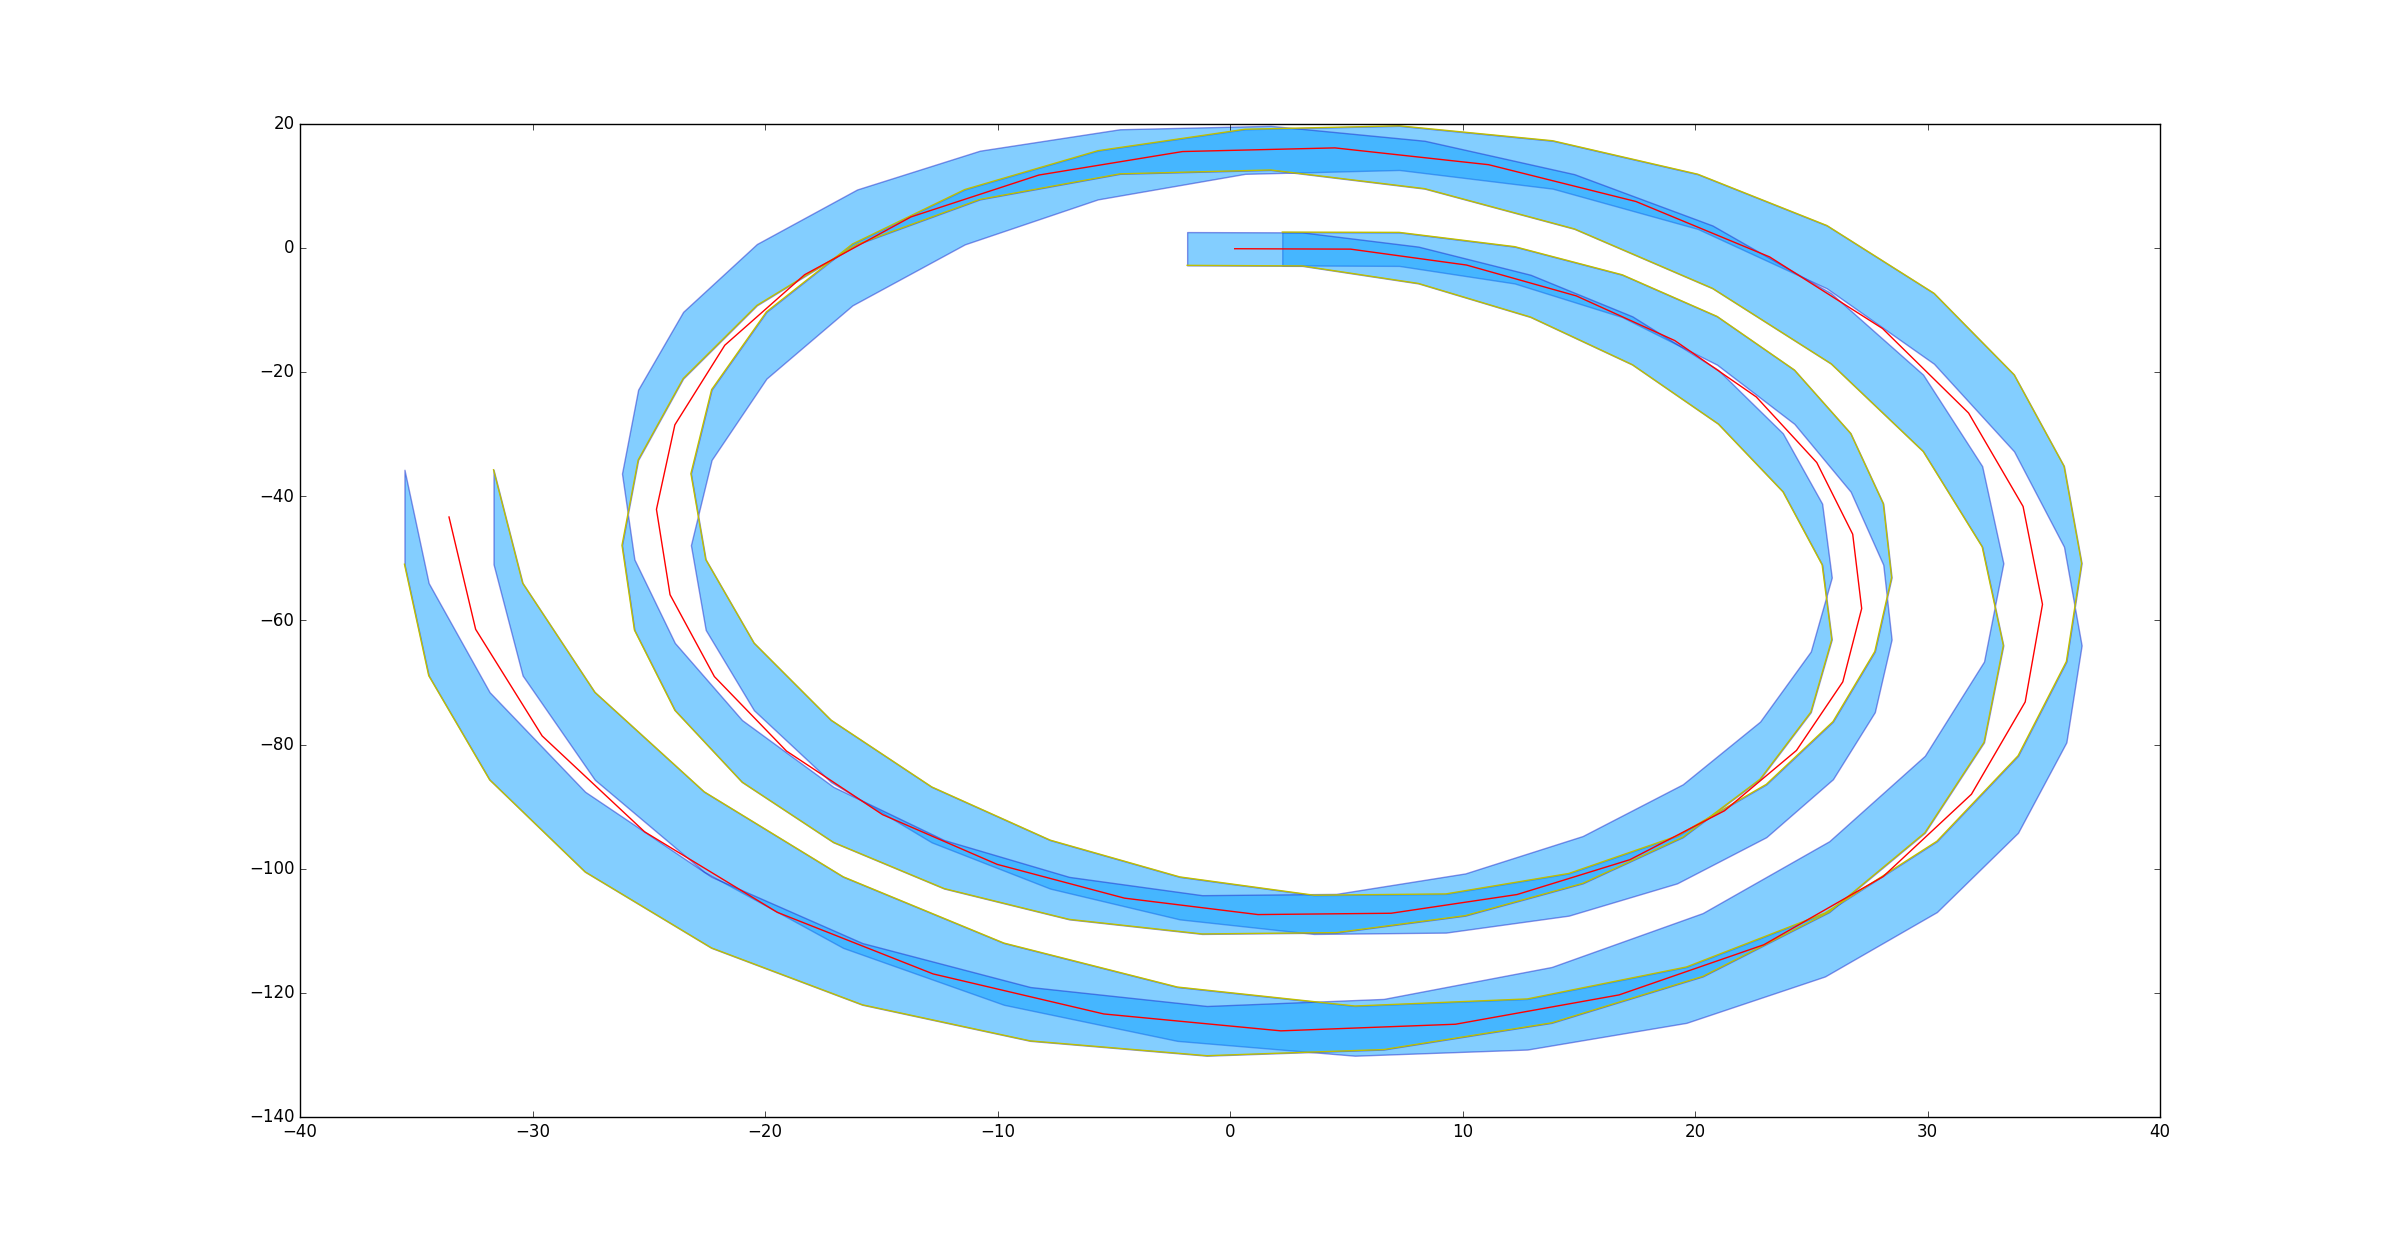
\includegraphics[scale=0.35,trim=70mm 0mm 0mm 0mm,clip=true]{states_a.png}
The Actions are oscillating as aspected for such an spiral trajectory.\\
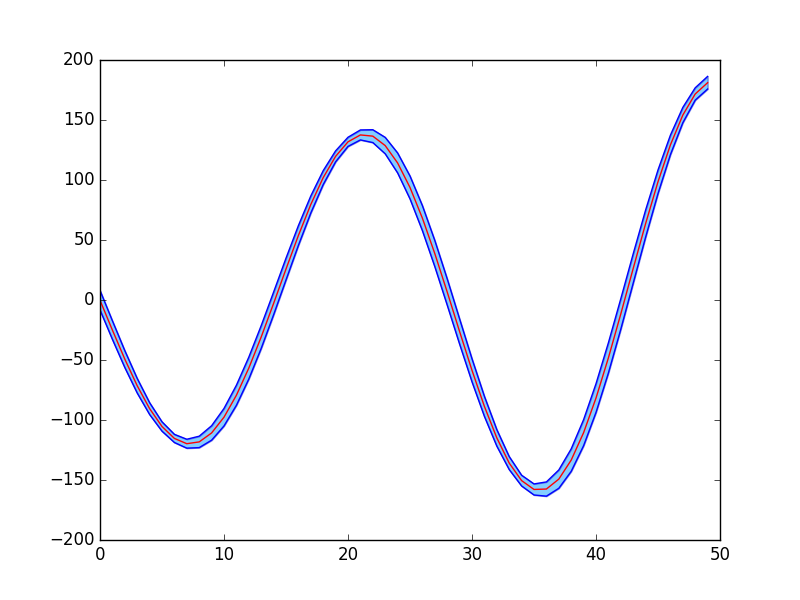
\includegraphics[scale=0.35,trim=70mm 0mm 0mm 0mm,clip=true]{actions_a.png}
\newpage
negative cumulative reward:\\
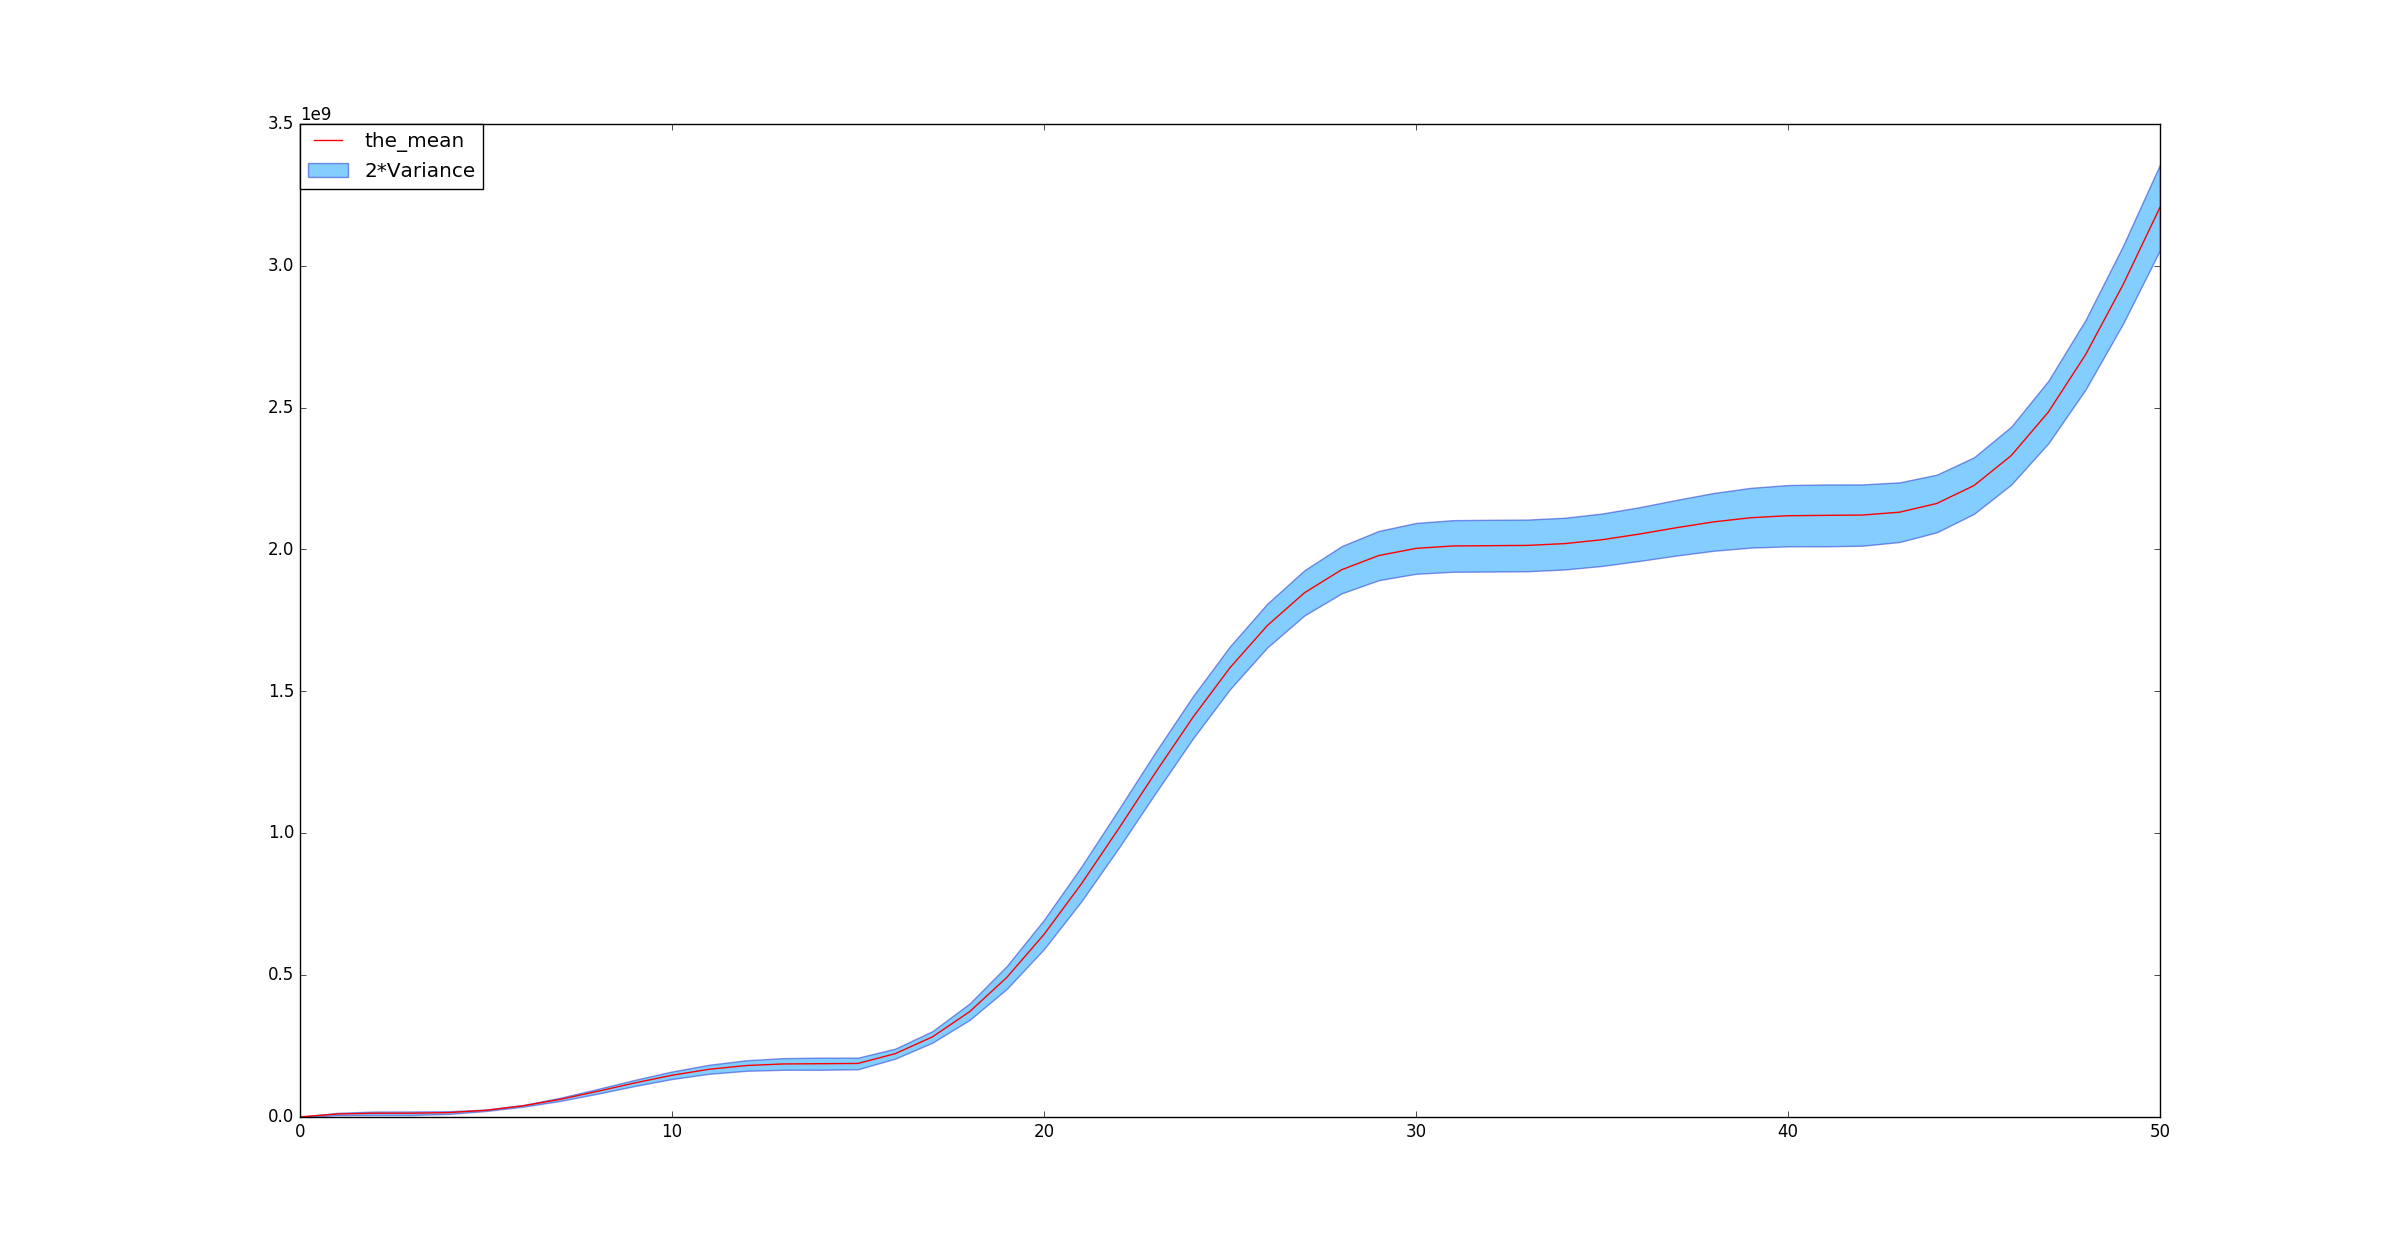
\includegraphics[scale=0.35,trim=70mm 0mm 0mm 0mm,clip=true]{rewards_a.png}
\newpage
\lstinputlisting[language=Python,breaklines=true]{lqr-1a.py}
\end{answer}


\end{question}

%---------------------------------

\begin{question}{LQR as a P controller}{4}

	The LQR can also be seen as a simple P controller of the form
	%
	\begin{align}
		\vec a_t = \mat K_t (\vec s^\text{des}_t - \vec s_t) + \vec k_t\,,
	\end{align}
	%
	which corresponds to the controller used in the canonical LQR system with the introduction of the target $\vec s^\text{des}_t$.
	
	Assume as target 
	\begin{align}
        \vec s^\text{des}_t = \vec r_t = \begin{cases}
        \begin{bmatrix}
        10\\
        0
        \end{bmatrix}  & \text{if \quad} t=0,1,\ldots,14
        \\
        \begin{bmatrix}
        20\\
        0
        \end{bmatrix}  & \text{if \quad} t=15,16,\ldots,T
        \end{cases}	
	\end{align}
    
    Use the same LQR system as in the previous exercise and run 20 experiments. Plot in one figure the mean and 95\% confidence of the first state, for both $\vec s^\text{des}_t = \vec r_t$ and $\vec s^\text{des}_t = \vec 0$.

\begin{answer}
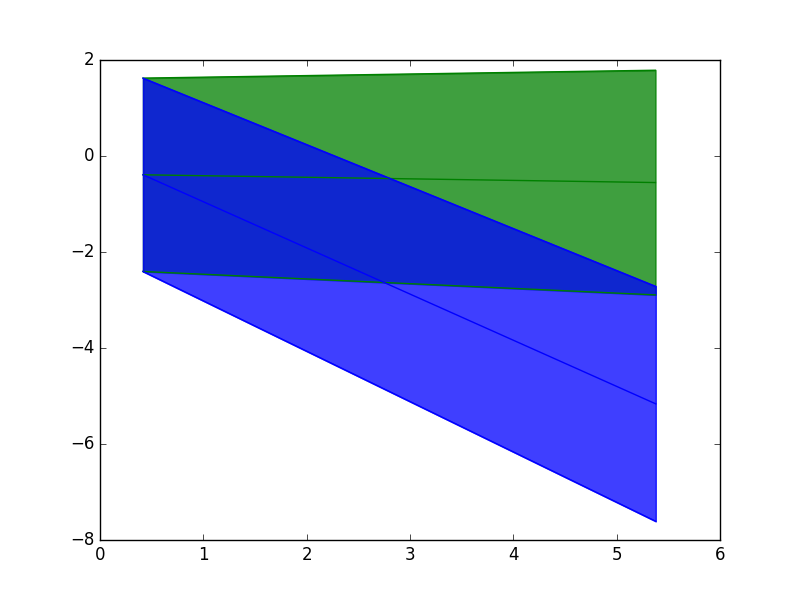
\includegraphics[scale=0.35,trim=0mm 0mm 0mm 0mm,clip=true]{states_b.png}
\end{answer}
\end{question}

%---------------------------------
	
	
\begin{question}{Optimal LQR}{8}
	To compute the optimal gains $\mat K_t$ and $\vec k_t$, which maximize the cumulative reward, we can use an analytic optimal solution. This controller recursively computes the optimal action by
	\begin{align}
		\vec a^* &= -(\mat H_t + \mat B^T_t \mat V_{t+1}\mat B_t)^{-1}	\mat B^T_t (\mat V_{t+1} (\mat A_t \vec s_t+\mat b_t )- \vec v_{t+1} ),
	\end{align}
	which can be decomposed into
	\begin{align}
		\mat K_t &= -(\mat H_t + \mat B^T_t \mat V_{t+1}\mat B_t)^{-1}	\mat B^T_t \mat V_{t+1} \mat A_t,
		\\
		\mat k_t &= -(\mat H_t + \mat B^T_t \mat V_{t+1}\mat B_t)^{-1}	\mat B^T_t (\mat V_{t+1} \mat b_t - \vec v_{t+1}).
	\end{align}
	%
	where
	%
	\begin{align}
		\mat M_t &= \mat B_t(\mat H_t + \mat B^T_t \mat V_{t+1}\mat B_t)^{-1}	\mat B^T_t \mat V_{t+1} \mat A_t
		\\
		\mat V_t &=
		\begin{cases}
	       \mat R_t + (\mat A_t - \mat M_t)^T\mat V_{t+1}\mat A_t & \text{when \quad} t = 1...T-1
	       \\
	       \mat R_t & \text{when \quad} t = T
	    \end{cases}
	    \\
		\mat v_t &= 
		\begin{cases}
	       \mat R_t\vec r_t + (\mat A_t - \mat M_t)^T(\vec v_{t+1} - \mat V_{t+1}\mat b_t) & \text{when \quad} t = 1...T-1
	       \\
	       \mat R_t\vec r_t & \text{when \quad} t = T
	    \end{cases}
	\end{align}		 

	Run 20 experiments with $\vec s^\text{des}_t = \vec 0$ computing the optimal gains $\mat K_t$ and $\vec k_t$. Plot the mean and 95\% confidence of both states for all three different controllers used so far. Use one figure per state. 
	Report the mean and std of the cumulative reward for each controller and comment the results. Attach a snippet of your code.

\begin{answer}
The contoller of 1c) has a much higher Variance than the others.\\
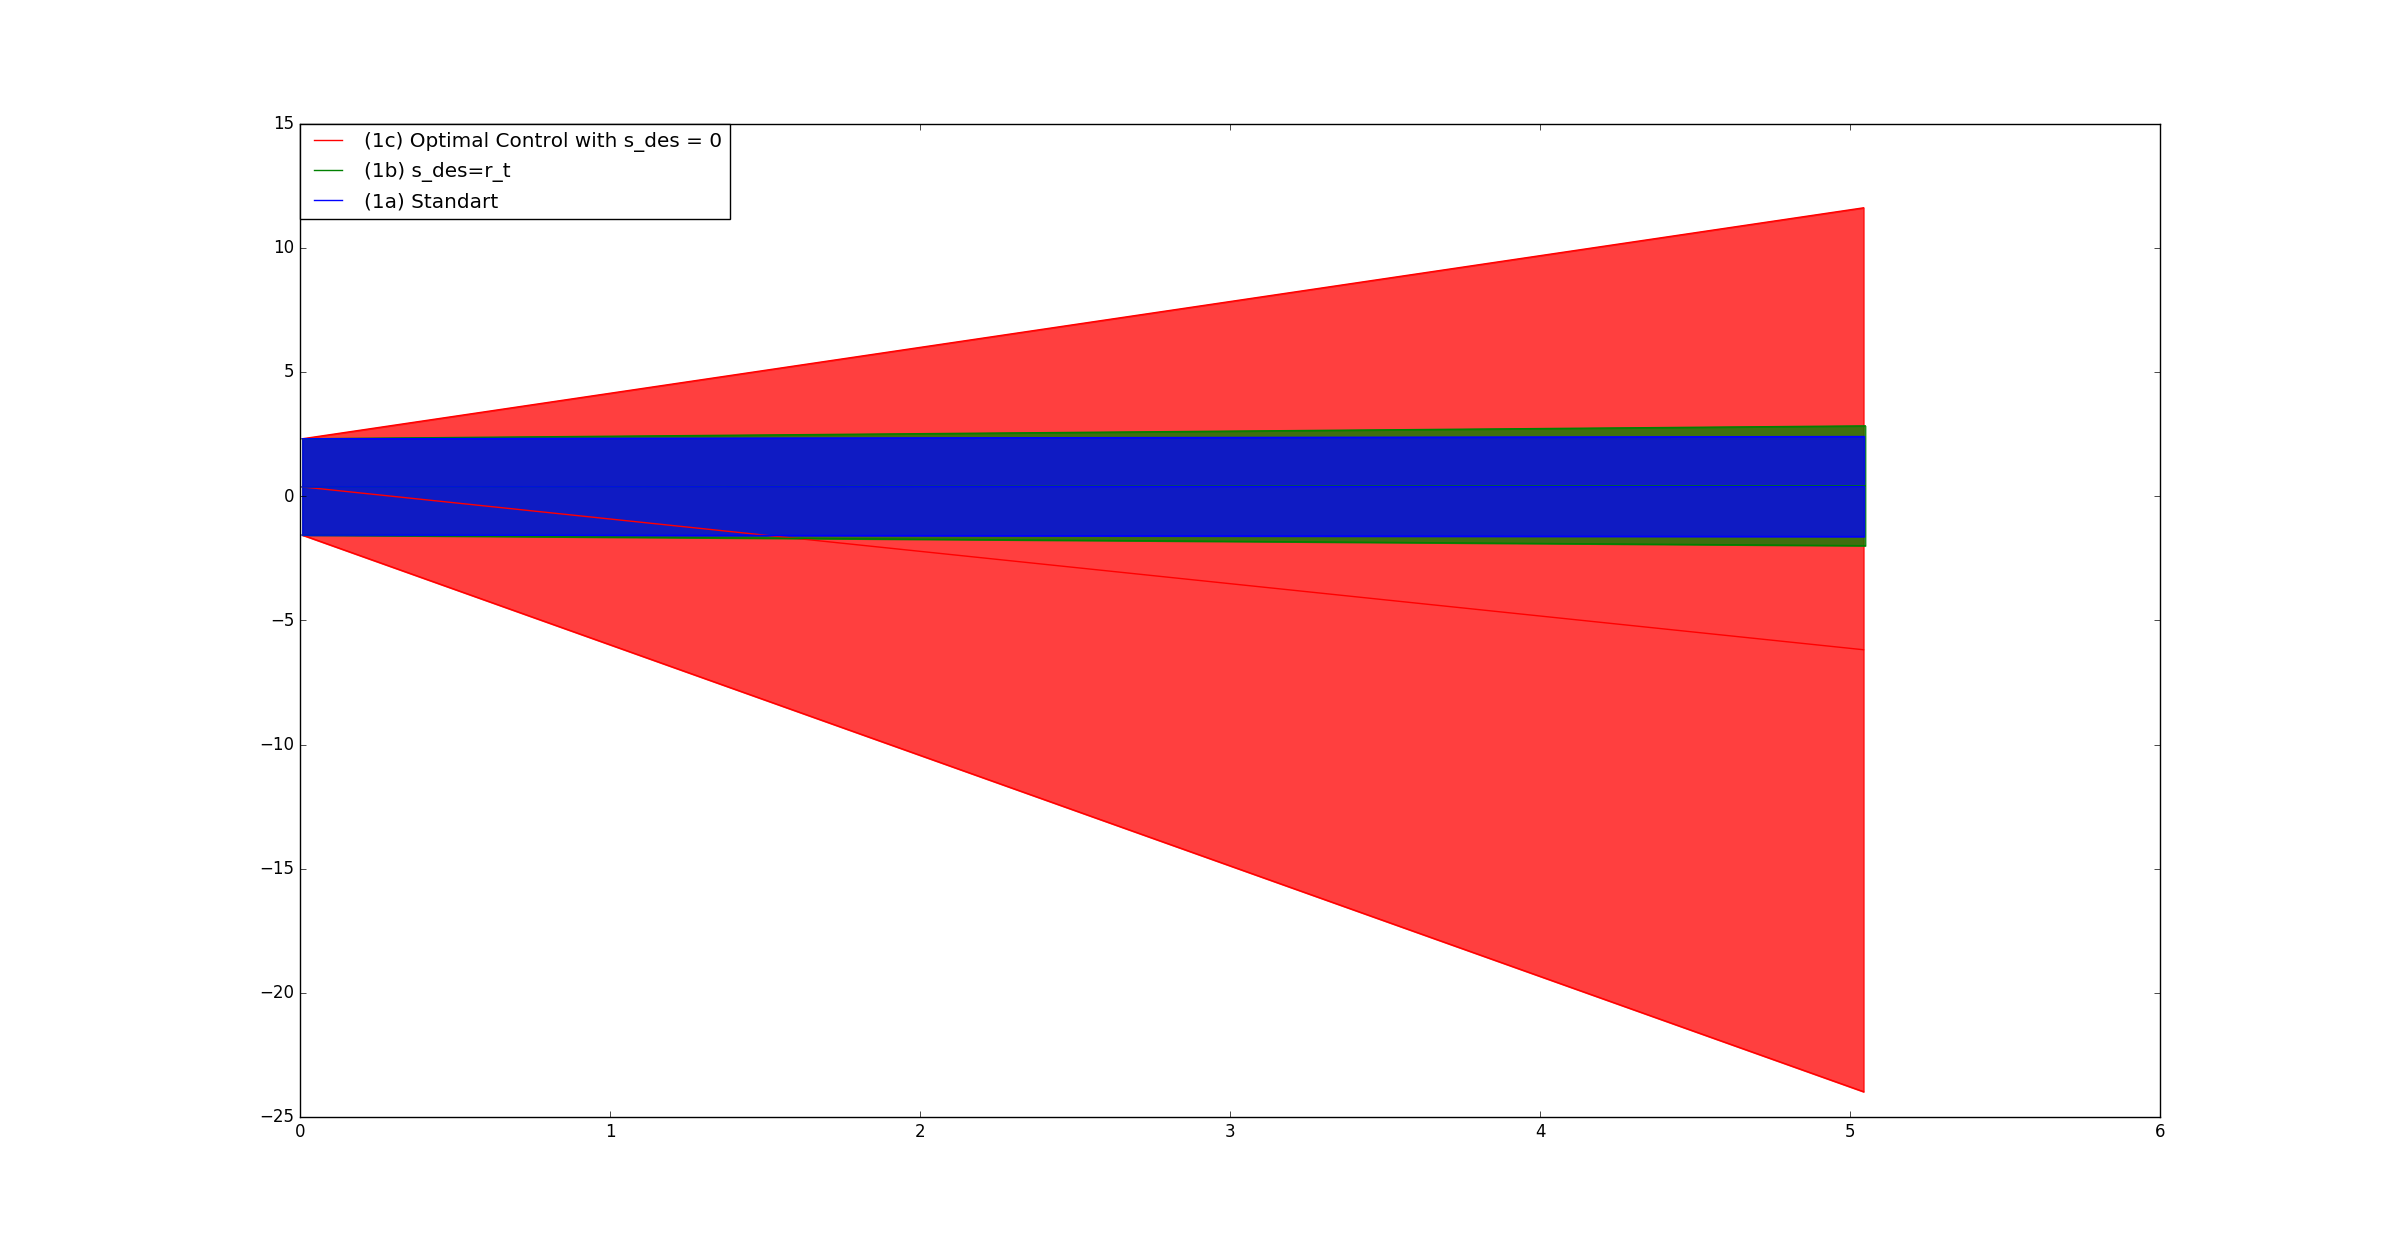
\includegraphics[scale=0.35,trim=70mm 0mm 0mm 0mm,clip=true]{states_c2.png}
As you can see rewards for 1c) are way too big, therefore we plot 1a) and 1b) together again (voilet = red+ blue)\\
negative cumulative reward:\\
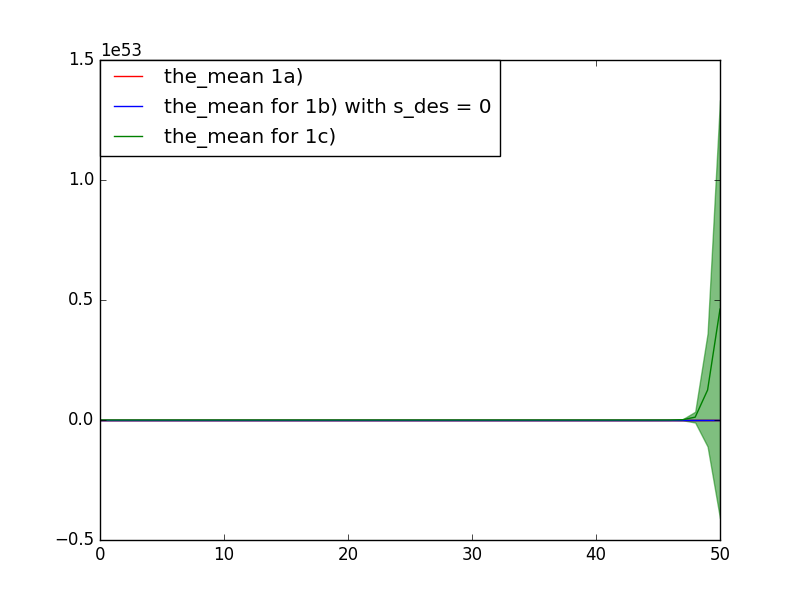
\includegraphics[scale=0.35,trim=0mm 0mm 0mm 0mm,clip=true]{rewards_c.png}
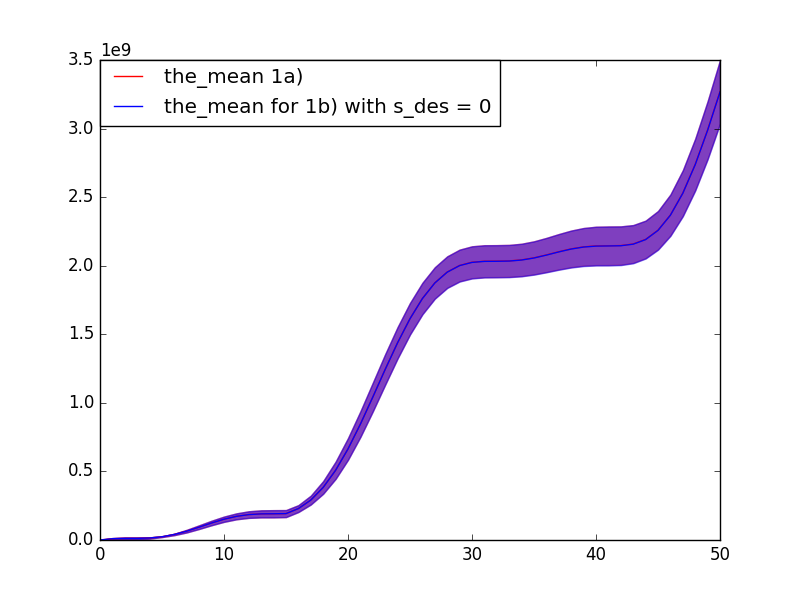
\includegraphics[scale=0.35,trim=0mm 0mm 0mm 0mm,clip=true]{rewards_c2.png}\newpage
\lstinputlisting[language=Python,breaklines=true]{lqr-1a.py}
\end{answer}

\end{question}

%----------------------------------------------

\end{questions}
